\chapter{پیشینه پژوهش}\label{chp2}

در فصل پیش، مفاهیم پایه‌ای مدل‌های مولد، مدل‌های انتشار و مبدل‌های بینایی در سطح مقدماتی معرفی شد. در این فصل، تمرکز از تعریف اولیه به سمت چارچوب‌های پژوهشی و مسیر تکامل مدل‌های انتشار می‌رود؛ به‌گونه‌ای که ابتدا فرمول‌بندی‌های اصلی این خانواده از مدل‌ها، شامل \lr{DDPM}، مدل‌های مبتنی بر امتیاز، فرمول‌بندی پیوسته و روش‌های نمونه‌برداری مرور می‌شوند. سپس نشان داده می‌شود که چرا پس از تثبیت این چارچوب‌ها، انتخاب معماری شبکه حذف نویز اهمیت پیدا کرده و چگونه این مسیر به مدل‌های انتشار مبتنی بر مبدل، به‌ویژه \lr{DiT}، منتهی شده است. در ادامه، روندهای تکمیلی از نظر مقیاس‌پذیری، کنترل‌پذیری و حفظ جزئیات محلی بررسی می‌گردد. سپس معماری‌های جریان دوگانه و روش‌های تجمیع ویژگی مطالعه می‌شوند تا مبنای نظری شاخه وضوح‌بالای پیشنهادی روشن شود. در پایان نیز روش‌های تنظیم دقیق، به‌ویژه رویکردهای پارامتر-کارا، بررسی می‌شوند؛ زیرا معماری پیشنهادی این پژوهش بر ترکیب یک بدنه اصلی منجمد با یک شاخه جانبی آموزش‌پذیر استوار است \cite{0214306,2212.09748,chen2021crossvit,8409325}.

\section{چارچوب‌های اصلی مدل‌های انتشار}
\label{sec:ch2-diffusion-frameworks}
توضیح مقدماتی فصل پیش نشان داد که مدل انتشار از دو مسیر نویزدهی و حذف نویز تشکیل می‌شود. در پیشینه پژوهش، این ایده در چند فرمول‌بندی اصلی توسعه یافته است که هر یک زاویه متفاوتی از همان مسئله را برجسته می‌کنند: در \lr{DDPM}\LTRfootnote{Denoising Diffusion Probabilistic Models}، فرایند تولید به‌صورت یک زنجیره مارکوف گسسته مدل می‌شود؛ در مدل‌های مبتنی بر امتیاز، هدف یادگیری گرادیان لگاریتم چگالی داده‌های نویزی است؛ و در فرمول‌بندی پیوسته، هر دو نگاه در قالب معادلات دیفرانسیل تصادفی و معادلات دیفرانسیل معمولی قابل بیان می‌شوند \cite{sohlDickstein2015deepUnsupervised,ho2020ddpm,song2019scoreGenerative,song2021scoreSDE}. این بخش برای جلوگیری از تکرار فصل اول، بر تفاوت این چارچوب‌ها، روابط ریاضی کلیدی و جایگاه آن‌ها در تعریف نقش شبکه حذف نویز تمرکز دارد.

\subsection{مدل‌های \lr{DDPM}}
در فرمول‌بندی احتمالاتی، داده واقعی با $x_0 \sim q_{\text{data}}(x)$ نمایش داده می‌شود و یک زمان‌بندی نویز\LTRfootnote{Noise Schedule} شامل ضرایب $\{\beta_t\}_{t=1}^{T}$ مشخص می‌کند که در هر گام چه مقدار نویز گاوسی به داده افزوده شود. اگر $\alpha_t = 1-\beta_t$ و $\bar{\alpha}_t = \prod_{s=1}^{t}\alpha_s$ باشد، فرایند رو به جلو به صورت زیر نوشته می‌شود \cite{sohlDickstein2015deepUnsupervised,ho2020ddpm}:
\begin{equation}
q(x_t|x_{t-1}) = \mathcal{N}\left(x_t; \sqrt{\alpha_t}x_{t-1}, (1-\alpha_t)I\right).
\end{equation}
مزیت این تعریف آن است که نمونه نویزی در هر گام را می‌توان مستقیماً از $x_0$ نیز به دست آورد:
\begin{equation}
q(x_t|x_0) = \mathcal{N}\left(x_t; \sqrt{\bar{\alpha}_t}x_0, (1-\bar{\alpha}_t)I\right),
\end{equation}
یا به شکل بازپارامتری‌شده:
\begin{equation}
x_t = \sqrt{\bar{\alpha}_t}x_0 + \sqrt{1-\bar{\alpha}_t}\epsilon,\quad \epsilon \sim \mathcal{N}(0,I).
\end{equation}
بنابراین، آموزش مدل به معنای یادگیری مسیر معکوس از $x_t$ به $x_{t-1}$ است:
\begin{equation}
p_\theta(x_{t-1}|x_t) = \mathcal{N}\left(x_{t-1}; \mu_\theta(x_t,t), \Sigma_\theta(x_t,t)\right).
\end{equation}
در \lr{DDPM}، به‌جای پیش‌بینی مستقیم $x_{t-1}$، شبکه معمولاً نویز افزوده‌شده را تخمین می‌زند. این انتخاب باعث می‌شود تابع هدف عملی به یک خطای میانگین مربعات ساده تبدیل شود \cite{ho2020ddpm}:
\begin{equation}
\mathcal{L}_{\text{\lr{DDPM}}} =
\mathbb{E}_{x_0,\epsilon,t}
\left[
\left\|
\epsilon - \epsilon_\theta(x_t,t,c)
\right\|_2^2
\right],
\end{equation}
که در آن $c$ می‌تواند شرطی مانند برچسب کلاس یا متن باشد. همین رابطه در مدل‌های مبتنی بر \lr{DiT} نیز حفظ می‌شود؛ تفاوت اصلی در آن است که تابع $\epsilon_\theta$ به‌جای یک شبکه پیچشی، با یک معماری مبدلی پیاده‌سازی می‌شود \cite{2212.09748}.

\subsection{مدل‌های مبتنی بر امتیاز}
دیدگاه مبتنی بر امتیاز\LTRfootnote{Score-Based Modeling} مسئله را از زاویه دیگری بیان می‌کند. در این رویکرد، مدل به‌جای تخمین مستقیم چگالی داده، تابع امتیاز توزیع داده‌های نویزی را یاد می‌گیرد \cite{song2019scoreGenerative,song2021scoreSDE}:
\begin{equation}
s_\theta(x_t,t) \approx \nabla_{x_t}\log q_t(x_t).
\end{equation}
تابع امتیاز جهت افزایش احتمال داده را در فضای نمونه نشان می‌دهد؛ به بیان دیگر، مشخص می‌کند یک نمونه نویزی باید در چه جهتی حرکت کند تا به نواحی محتمل‌تر توزیع داده نزدیک شود. ارتباط این دیدگاه با \lr{DDPM} از رابطه نویز گاوسی روشن می‌شود. اگر $\sigma_t^2 = 1-\bar{\alpha}_t$ باشد، امتیاز توزیع شرطی نویزی با نویز افزوده‌شده نسبت مستقیم دارد:
\begin{equation}
\nabla_{x_t}\log q(x_t|x_0) = -\frac{\epsilon}{\sigma_t}.
\end{equation}
بنابراین، پیش‌بینی نویز در \lr{DDPM} و تخمین امتیاز در مدل‌های مبتنی بر امتیاز دو بیان نزدیک از یک مسئله هستند. این ارتباط اهمیت زیادی دارد، زیرا نشان می‌دهد روش‌های مختلف مدل‌های انتشار تنها نام‌گذاری‌های جداگانه نیستند، بلکه از نظر ریاضی به یک خانواده مشترک تعلق دارند \cite{song2021scoreSDE,0214306}.

\subsection{مدل‌های انتشار مبتنی بر \lr{SDE}}
برای یکپارچه‌سازی دیدگاه‌های گسسته و مبتنی بر امتیاز، مدل‌های انتشار را می‌توان در زمان پیوسته با معادله دیفرانسیل تصادفی\LTRfootnote{Stochastic Differential Equation} بیان کرد \cite{song2021scoreSDE}:
\begin{equation}
d x = f(x,t)\,dt + g(t)\,d w,
\end{equation}
که در آن $f(x,t)$ جمله رانش، $g(t)$ شدت نویز و $w$ فرایند وینر است. در مسیر رو به جلو، این معادله داده را به‌تدریج به توزیع ساده‌ای مانند نرمال استاندارد نزدیک می‌کند. مسیر معکوس نیز با استفاده از تابع امتیاز قابل نوشتن است:
\begin{equation}
d x =
\left[
f(x,t) - g(t)^2\nabla_x\log p_t(x)
\right]dt
+ g(t)\,d\bar{w}.
\end{equation}
این رابطه نشان می‌دهد که اگر مدل بتواند امتیاز $\nabla_x\log p_t(x)$ را تخمین بزند، می‌توان مسیر تولید را از نویز به داده طی کرد. همچنین یک معادله دیفرانسیل معمولی\LTRfootnote{Ordinary Differential Equation} متناظر، موسوم به \lr{Probability Flow ODE}، وجود دارد:
\begin{equation}
\frac{d x}{dt} =
f(x,t) - \frac{1}{2}g(t)^2\nabla_x\log p_t(x).
\end{equation}
این نگاه پیوسته برای طراحی نمونه‌بردارهای سریع‌تر و تحلیل ارتباط میان خانواده‌های مختلف مدل‌های انتشار اهمیت دارد؛ زیرا انتخاب زمان‌بندی نویز، گام‌های حل عددی و پارامترسازی شبکه را از یکدیگر تفکیک می‌کند \cite{song2021scoreSDE,karras2022edm}.

\subsection{نمونه‌برداری، \lr{DDIM} و هدایت تولید}
یکی از محدودیت‌های اولیه مدل‌های انتشار، نیاز به تعداد زیاد گام‌های نمونه‌برداری بود. \lr{DDIM}\LTRfootnote{Denoising Diffusion Implicit Models} نشان داد که می‌توان با تعریف یک مسیر غیرمارکوفی، نمونه‌برداری را با گام‌های کمتر انجام داد، در حالی که از همان شبکه آموزش‌دیده استفاده می‌شود \cite{song2021ddim}. ابتدا تخمین تصویر پاک از روی نمونه نویزی محاسبه می‌شود:
\begin{equation}
\hat{x}_0 =
\frac{x_t - \sqrt{1-\bar{\alpha}_t}\epsilon_\theta(x_t,t,c)}
{\sqrt{\bar{\alpha}_t}}.
\end{equation}
سپس نمونه گام قبلی با ترکیب $\hat{x}_0$ و نویز پیش‌بینی‌شده ساخته می‌شود. در حالت کلی:
\begin{equation}
x_{t-1} =
\sqrt{\bar{\alpha}_{t-1}}\hat{x}_0
+ \sqrt{1-\bar{\alpha}_{t-1}-\sigma_t^2}\epsilon_\theta(x_t,t,c)
+ \sigma_t z,
\end{equation}
که در آن $z \sim \mathcal{N}(0,I)$ است. با انتخاب $\sigma_t=0$، فرایند نمونه‌برداری قطعی می‌شود و می‌تواند با تعداد گام کمتر اجرا گردد. در مدل‌های شرطی، علاوه بر سرعت نمونه‌برداری، کنترل خروجی نیز اهمیت دارد. یکی از روش‌های رایج برای افزایش کنترل‌پذیری، هدایت تولید است؛ به این معنا که مسیر حذف نویز فقط از توزیع کلی داده پیروی نکند، بلکه به سمت شرط مورد نظر، مانند برچسب کلاس، سوق داده شود. روش‌های اولیه هدایت معمولاً به یک طبقه‌بند جداگانه نیاز داشتند تا در هر گام نمونه‌برداری گرادیان احتمال کلاس را محاسبه کند. در مقابل، راهنمایی بدون طبقه‌بند\LTRfootnote{Classifier-Free Guidance} یا \lr{CFG} این وابستگی را حذف می‌کند و همان شبکه حذف نویز را هم برای پیش‌بینی شرطی و هم برای پیش‌بینی بی‌شرط به کار می‌گیرد \cite{ho2022classifierFreeGuidance}.

برای ممکن شدن این کار، در زمان آموزش، شرط $c$ با احتمالی مشخص حذف و با شرط تهی $\emptyset$ جایگزین می‌شود. بنابراین مدل واحد $\epsilon_\theta$ یاد می‌گیرد هم نویز را در حالت شرطی، یعنی $\epsilon_\theta(x_t,t,c)$، و هم در حالت بی‌شرط، یعنی $\epsilon_\theta(x_t,t,\emptyset)$، تخمین بزند. در زمان نمونه‌برداری، این دو پیش‌بینی با یکدیگر ترکیب می‌شوند:
\begin{equation}
\epsilon_{\text{\lr{cfg}}} =
\epsilon_\theta(x_t,t,\emptyset)
+ w\left(
\epsilon_\theta(x_t,t,c) -
\epsilon_\theta(x_t,t,\emptyset)
\right),
\end{equation}
که در آن $w$ شدت هدایت را کنترل می‌کند. اختلاف
$\epsilon_\theta(x_t,t,c)-\epsilon_\theta(x_t,t,\emptyset)$
را می‌توان جهت اثر شرط دانست؛ یعنی بخشی از پیش‌بینی نویز که به حضور شرط وابسته است. وقتی $w=0$ باشد، نمونه‌برداری عملاً بی‌شرط است. وقتی $w=1$ باشد، خروجی معادل پیش‌بینی شرطی معمولی می‌شود. برای مقادیر بزرگ‌تر از یک، نمونه‌بردار در جهت شرط فراتر از پیش‌بینی شرطی حرکت می‌کند و در نتیجه تصویر معمولاً نشانه‌های معنایی مرتبط با کلاس را واضح‌تر نشان می‌دهد.

تأثیر \lr{CFG} دوگانه است. از یک سو، افزایش $w$ می‌تواند وفاداری شرطی\LTRfootnote{Conditional Fidelity} را بهبود دهد؛ برای مثال، در تولید کلاسی \lr{ImageNet} احتمال اینکه نمونه تولیدشده واقعاً با کلاس خواسته‌شده سازگار باشد بیشتر می‌شود. از سوی دیگر، اگر ضریب هدایت بیش از حد بزرگ شود، مدل به ناحیه محدودتری از توزیع داده رانده می‌شود. این موضوع می‌تواند تنوع نمونه‌ها را کاهش دهد، بافت‌ها را بیش از حد تیز یا اشباع کند، و حتی معیارهای توزیعی مانند \lr{FID} و \lr{KID} را بدتر کند. بنابراین \lr{CFG} یک اهرم تنظیم بین وفاداری به شرط و تنوع توزیعی است، نه یک بهبود بدون هزینه. از نظر محاسباتی نیز نمونه‌برداری با \lr{CFG} معمولاً به دو پیش‌بینی شرطی و بی‌شرط در هر گام نیاز دارد و هزینه استنتاج شبکه حذف نویز را افزایش می‌دهد، هرچند به آموزش یا نگهداری طبقه‌بند جداگانه احتیاج ندارد \cite{ho2022classifierFreeGuidance}.

این رابطه برای این پایان‌نامه مهم است، زیرا ارزیابی اصلی روی تولید شرطی \lr{ImageNet-1K} انجام می‌شود و لازم است نمونه‌ها علاوه بر کیفیت بصری، به برچسب کلاس انتخاب‌شده نیز وفادار باشند. در فصل آزمایش‌ها، مقدار \lr{CFG} به‌عنوان یک ابرپارامتر نمونه‌برداری گزارش و تحلیل می‌شود تا اثر آن از اثر تغییرات معماری \lr{DuoDiT} جدا بماند.

\begin{table}[htbp]
    \centering
    \caption[مقایسه چارچوب‌های اصلی مدل‌های انتشار]{مقایسه چارچوب‌های اصلی مدل‌های انتشار}
    \label{tab:ch2-diffusion-frameworks}
    \resizebox{\textwidth}{!}{%
    \begin{tabular}{p{0.22\textwidth}p{0.38\textwidth}p{0.32\textwidth}}
        \hline
        \textbf{چارچوب} & \textbf{ایده اصلی} & \textbf{رابطه یا هدف کلیدی} \\
        \hline
        \lr{DDPM} & مدل‌سازی گسسته مسیر نویزدهی و حذف نویز & پیش‌بینی $\epsilon_\theta(x_t,t,c)$ با خطای میانگین مربعات \\
        مدل‌های مبتنی بر امتیاز & یادگیری گرادیان لگاریتم چگالی داده‌های نویزی & $s_\theta(x_t,t) \approx \nabla_{x_t}\log q_t(x_t)$ \\
        \lr{SDE/ODE} & بیان پیوسته فرایند نویزدهی و تولید & $dx=f(x,t)dt+g(t)dw$ \\
        \lr{DDIM} و نمونه‌بردارها & کاهش تعداد گام‌های تولید با مسیرهای جایگزین & بازسازی $\hat{x}_0$ از روی $x_t$ و $\epsilon_\theta$ \\
        \lr{CFG} & افزایش وفاداری شرطی در نمونه‌برداری بدون طبقه‌بند جداگانه & ترکیب $\epsilon_\theta(x_t,t,c)$ و $\epsilon_\theta(x_t,t,\emptyset)$ با ضریب $w$ \\
        \hline
    \end{tabular}%
    }
\end{table}

\section{مدل‌های انتشار مبتنی بر مبدل}
پس از تثبیت چارچوب‌های احتمالاتی، مبتنی بر امتیاز و پیوسته در مدل‌های انتشار، تمرکز پژوهش‌ها از تعریف فرایند حذف نویز به سمت طراحی معماری شبکه حذف نویز تغییر کرد؛ زیرا کیفیت تولید فقط به تابع هدف انتشار وابسته نیست و عواملی مانند فضای نمایش، زمان‌بندی نویز، نوع شرط‌گذاری، نمونه‌بردار و ساختار شبکه نیز در عملکرد نهایی اثر دارند \cite{0214306,7811582,9851474}. در همین مسیر، موفقیت مبدل‌ها در پردازش توالی و سپس در بینایی ماشین باعث شد پژوهشگران از معماری‌های مبتنی بر توجه برای مدل‌های مولد تصویری استفاده کنند \cite{Vaswani2017,Dosovitskiy2020}. برخلاف \lr{U-Net}ها و شبکه‌های پیچشی که سوگیری محلی قوی دارند، مبدل‌ها با مدل‌سازی وابستگی‌های دوربرد میان توکن‌های تصویری می‌توانند ساختار سراسری تصویر را بهتر دنبال کنند؛ هرچند نبود سوگیری محلی ذاتی، هزینه توجه و نیاز به حفظ جزئیات مکانی همچنان چالش‌های مهمی هستند \cite{0017415,3153255,9511279}. بنابراین، مسئله اصلی این بخش آن است که چگونه می‌توان نقش تابع $\epsilon_\theta$ را از یک بدنه اصلی پیچشی به یک معماری مبدلی منتقل کرد و در عین حال شرط زمانی، شرط کلاسی و اطلاعات مکانی تصویر را به‌صورت پایدار حفظ نمود \cite{2212.09748,5638143,8106348}.

\subsection{مدل \lr{GenViT}}
مدل \lr{GenViT}\LTRfootnote{Generative ViT} یکی از تلاش‌های اولیه برای بررسی این ایده بود که آیا می‌توان بدنه اصلی مدل انتشار را با یک \lr{ViT} خالص پیاده‌سازی کرد یا نه \cite{2208.07791}. اهمیت این مدل در آن است که پیش از تثبیت خانواده \lr{DiT}، امکان استفاده از توکن‌های تصویری و اطلاعات گام زمانی در یک معماری تمام‌مبدلی را بررسی کرد.

در \lr{GenViT}، توکن‌های تصویر نویزی همراه با اطلاعات زمان پردازش می‌شوند و تابع زیان، یادگیری تولیدی و تمایزگر را در کنار یکدیگر قرار می‌دهد:
\begin{equation}
\mathcal{L}_{\text{\lr{total}}} = \mathcal{L}_{\text{\lr{diff}}} + \lambda \mathcal{L}_{\text{\lr{cls}}}
\end{equation}
که در آن $\mathcal{L}_{\text{diff}}$ خطای بازسازی نویز و $\mathcal{L}_{\text{cls}}$ خطای دسته‌بندی است. این مدل از نظر تاریخی نشان می‌دهد که مبدل‌ها فقط برای استخراج ویژگی تصویری به کار نمی‌روند، بلکه می‌توانند در خود مسیر تولید نیز نقش داشته باشند. نمای کلی این معماری در شکل \ref{fig:genvit} نمایش داده شده است \cite{2208.07791}.

\begin{figure}[H]
	\centering
	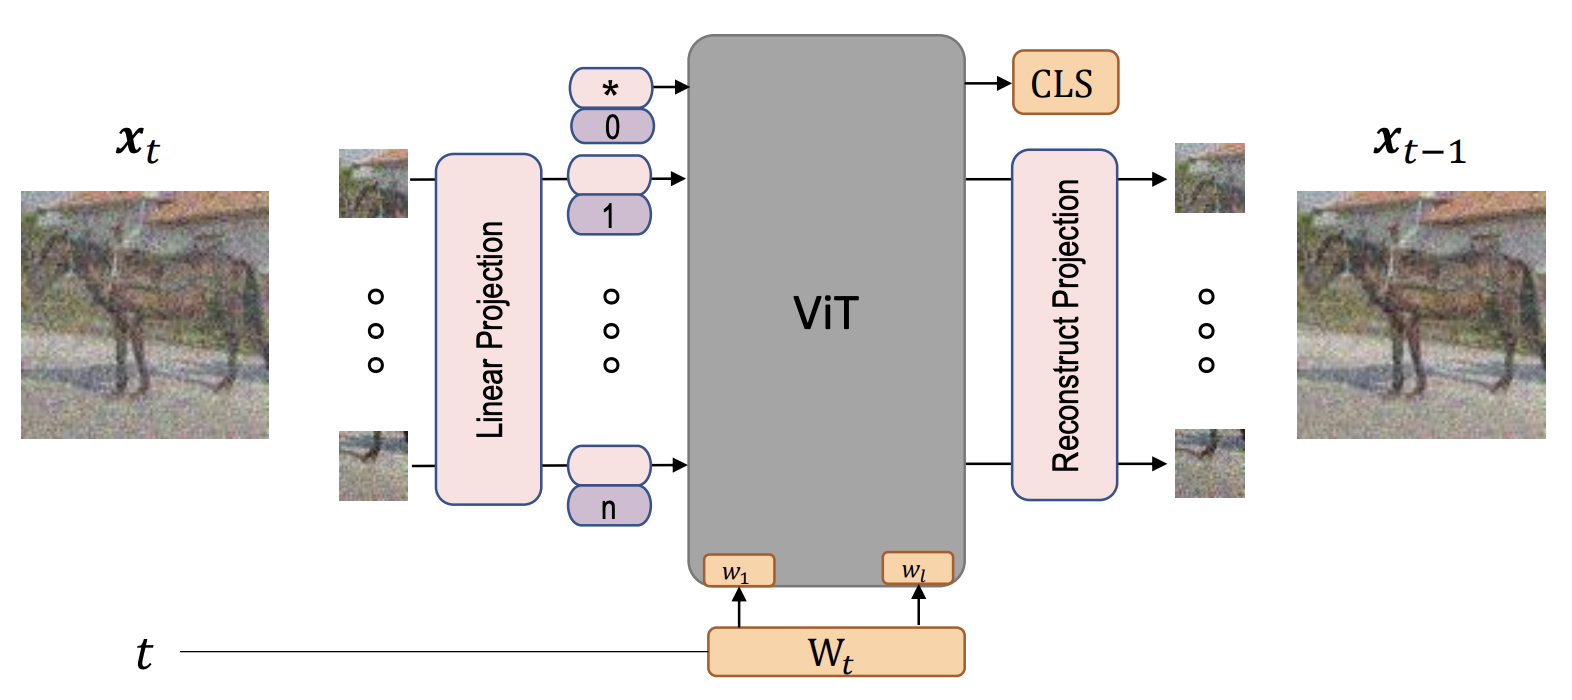
\includegraphics[width=0.9\textwidth]{images/gen_vit.png}
	\caption[معماری \lr{GenViT}]{معماری \lr{GenViT} که مبدل را در مدل انتشار ادغام می‌کند.}
	\label{fig:genvit}
\end{figure}

\subsection{مدل \lr{U-ViT}}
مدل \lr{U-ViT}\LTRfootnote{U-shaped Vision Transformer} مسئله دیگری را برجسته کرد: اگر شبکه حذف نویز کاملاً مبدلی باشد، چگونه می‌توان اطلاعات سطح پایین و جزئیات مکانی را در مسیر عمیق مدل حفظ کرد؟ بائو و همکاران با الهام از شکل \lr{U-Net}، اتصالات پرشی بلند\LTRfootnote{Long Skip Connections} را میان بلوک‌های کم‌عمق و عمیق مبدل وارد کردند تا اطلاعات محلی در طول فرایند حذف نویز از بین نرود \cite{2209.12152}.

در \lr{U-ViT}، تصویر نویزی، زمان و شرط‌هایی مانند برچسب کلاس همگی به صورت توکن پردازش می‌شوند و تخمین نویز $\epsilon_\theta(x_t, t, c)$ توسط یک شبکه تمام‌مبدلی انجام می‌گیرد. شکل \ref{fig:uvit} ساختار کلی این مدل را نشان می‌دهد. اهمیت \lr{U-ViT} برای این پایان‌نامه در آن است که نشان می‌دهد حتی در معماری‌های مبدلی نیز مسیرهای میان‌بر و چندسطحی برای حفظ جزئیات مکانی ضروری هستند \cite{2209.12152}.

\begin{figure}[H]
	\centering
	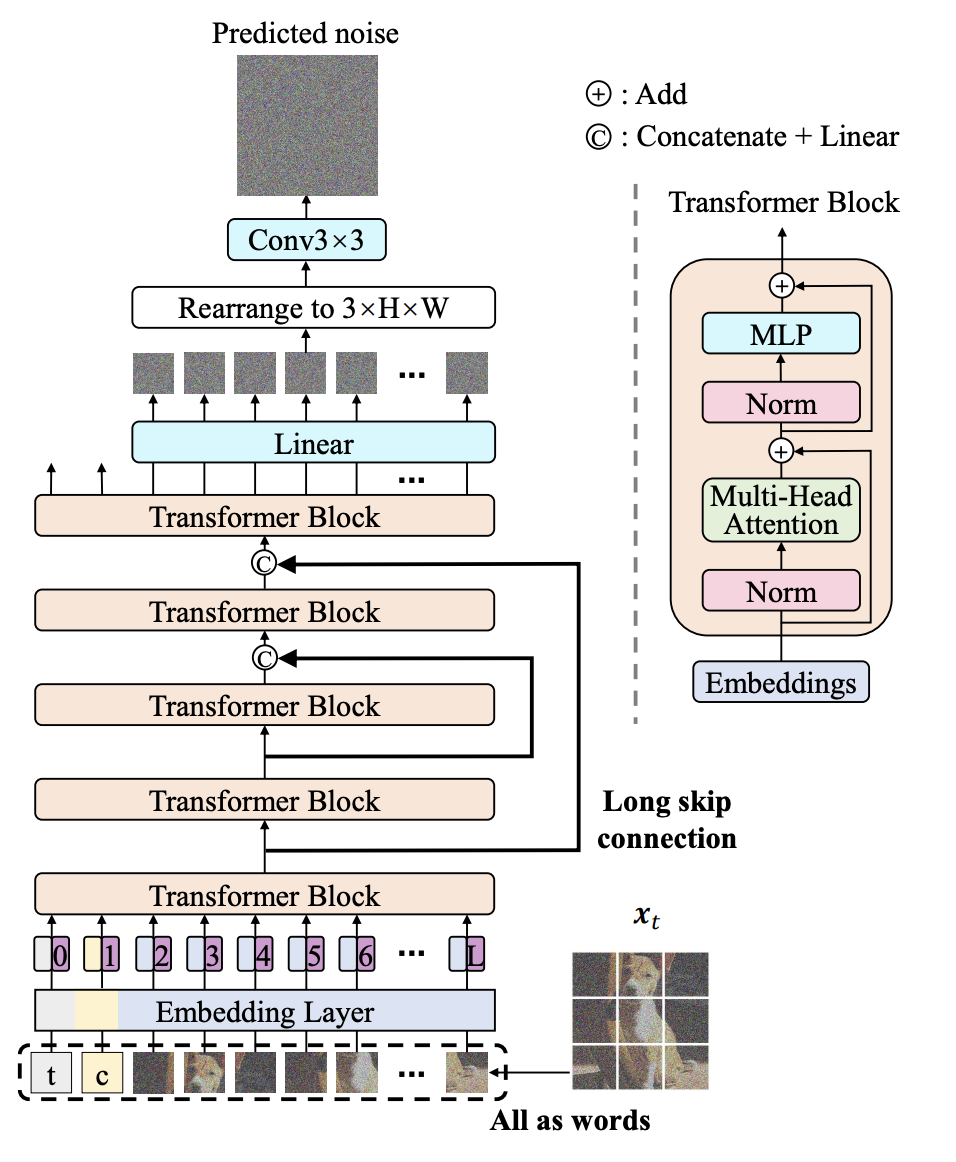
\includegraphics[width=0.9\textwidth]{images/u_vit.png}
	\caption[معماری \lr{U-ViT}]{معماری \lr{U-ViT} با اتصالات پرشی بلند بین بلوک‌های مبدل \cite{2209.12152}.}
	\label{fig:uvit}
\end{figure}

\subsection{مدل \lr{DiT}}
مدل مبدل انتشار\LTRfootnote{Diffusion Transformer} (\lr{DiT}) نقطه محوری این فصل است، زیرا نشان می‌دهد در مدل انتشار می‌توان معماری حذف نویز را از \lr{U-Net} به یک بدنه اصلی تمام‌مبدلی منتقل کرد، بدون آن‌که فرمول‌بندی انتشار تغییر کند \cite{2212.09748}. این مدل روی فضای نهان\LTRfootnote{Latent Space} عمل می‌کند؛ یعنی ابتدا تصویر به نمایش فشرده‌تری تبدیل می‌شود و سپس این نمایش به پچ‌ها و توکن‌ها شکسته می‌شود. پیبلز و شی نشان دادند که با افزایش تعداد پارامترها و حجم محاسبات، کیفیت تولید تصویر در این خانواده به‌صورت پیوسته بهبود می‌یابد.

معماری \lr{DiT} از بلوک‌های استاندارد \lr{ViT} استفاده می‌کند، اما برای تزریق اطلاعات زمان و کلاس از نرمال‌سازی لایه تطبیقی با مقداردهی صفر (\lr{adaLN-Zero}\LTRfootnote{Adaptive Layer Normalization with Zero Initialization}) بهره می‌برد. در این سازوکار، پارامترهای مقیاس ($\gamma$) و انتقال ($\beta$) در لایه‌های نرمال‌سازی از بردار زمان و کلاس پیش‌بینی می‌شوند:
\begin{equation}
\text{\lr{adaLN}}(h, t, c) = \gamma(t, c) \odot \text{\lr{Norm}}(h) + \beta(t, c)
\end{equation}
این روش، شرط‌گذاری را درون بلوک‌های مبدل وارد می‌کند و به مدل اجازه می‌دهد فرایند حذف نویز را در فضای فشرده‌تری نسبت به پیکسل‌ها انجام دهد. شکل \ref{fig:dit} ساختار کلی این معماری را نشان می‌دهد \cite{2212.09748}. از آنجا که معماری پیشنهادی این پایان‌نامه نیز یک شاخه مکمل را در کنار بدنه اصلی \lr{DiT} قرار می‌دهد، این مدل مرجع اصلی برای تحلیل‌های بعدی فصل است.

\begin{figure}[H]
	\centering
	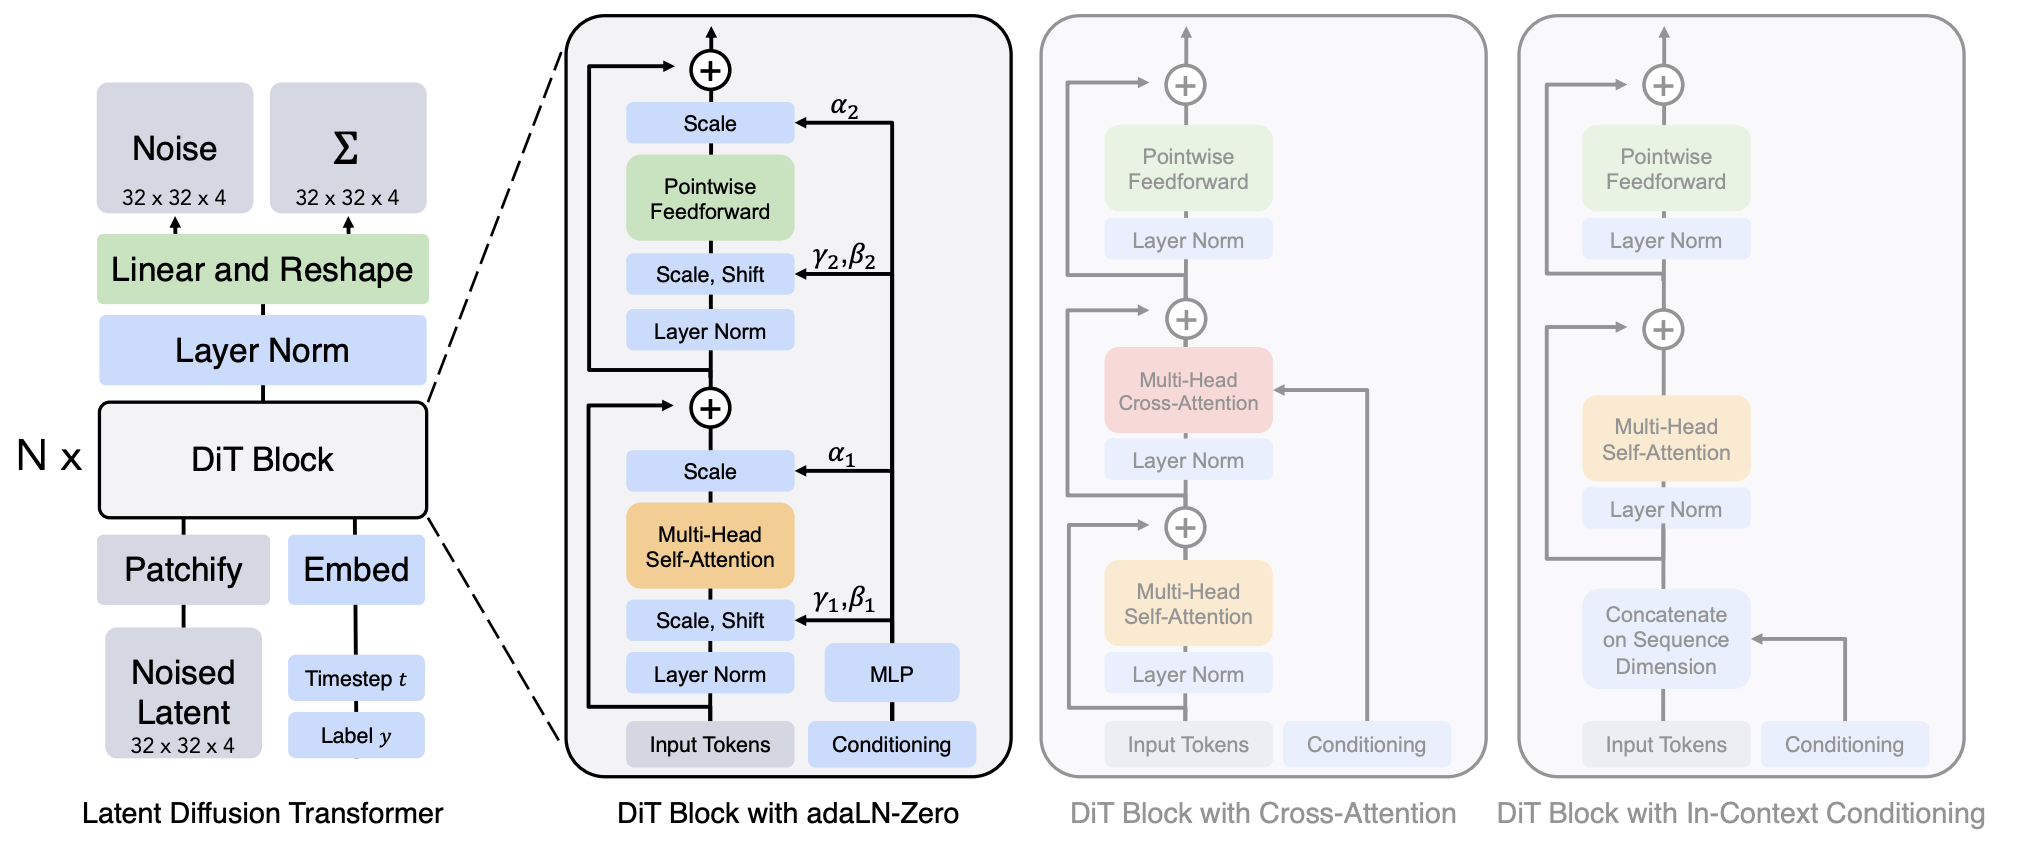
\includegraphics[width=0.9\textwidth]{images/base_dit.png}
	\caption[معماری \lr{DiT}]{معماری \lr{DiT} مبتنی بر بلوک‌های استاندارد مبدل و \lr{adaLN}.}
	\label{fig:dit}
\end{figure}

مدل \lr{DiffiT}\LTRfootnote{Diffusion Vision Transformer} بر محدودیت دیگری در مبدل‌های انتشار تمرکز دارد: نحوه وارد کردن زمان در فرایند توجه \cite{2312.02139v3}. در \lr{DiT}، زمان و کلاس عمدتاً از مسیر نرمال‌سازی تطبیقی وارد بلوک‌ها می‌شوند، اما \lr{DiffiT} یک مکانیزم خود توجه وابسته به زمان\LTRfootnote{Time-Dependent Self-Attention - TMSA} معرفی می‌کند تا ماتریس‌های توجه نیز مستقیماً از گام زمانی اثر بگیرند.

در این مدل، توکن زمان به‌صورت پویا در لایه‌های توجه حضور دارد و رابطه توجه ضرب داخلی مقیاس‌شده، که در رابطه \ref{eq:scaled-dot-product-attention} معرفی شد، با پرسش، کلید و مقدار وابسته به زمان نوشته می‌شود:
\begin{equation}
\text{\lr{Attention}}(Q_t, K_t, V_t) = \text{\lr{softmax}}\left(\frac{Q_t K_t^T}{\sqrt{d_k}}\right) V_t
\end{equation}
که در آن $Q_t, K_t, V_t$ با استفاده از تعبیه‌های مکانی و زمانی مشترک محاسبه می‌شوند. این طراحی به مدل اجازه می‌دهد پویایی حذف نویز را با دقت بیشتری دنبال کند و در عین حال، با ساختار چندوضوحی خود بخشی از هزینه محاسباتی را کنترل نماید. شکل \ref{fig:diffit} نمایی از این ساختار را ارائه می‌کند \cite{2312.02139v3}.

\begin{figure}[H]
	\centering
	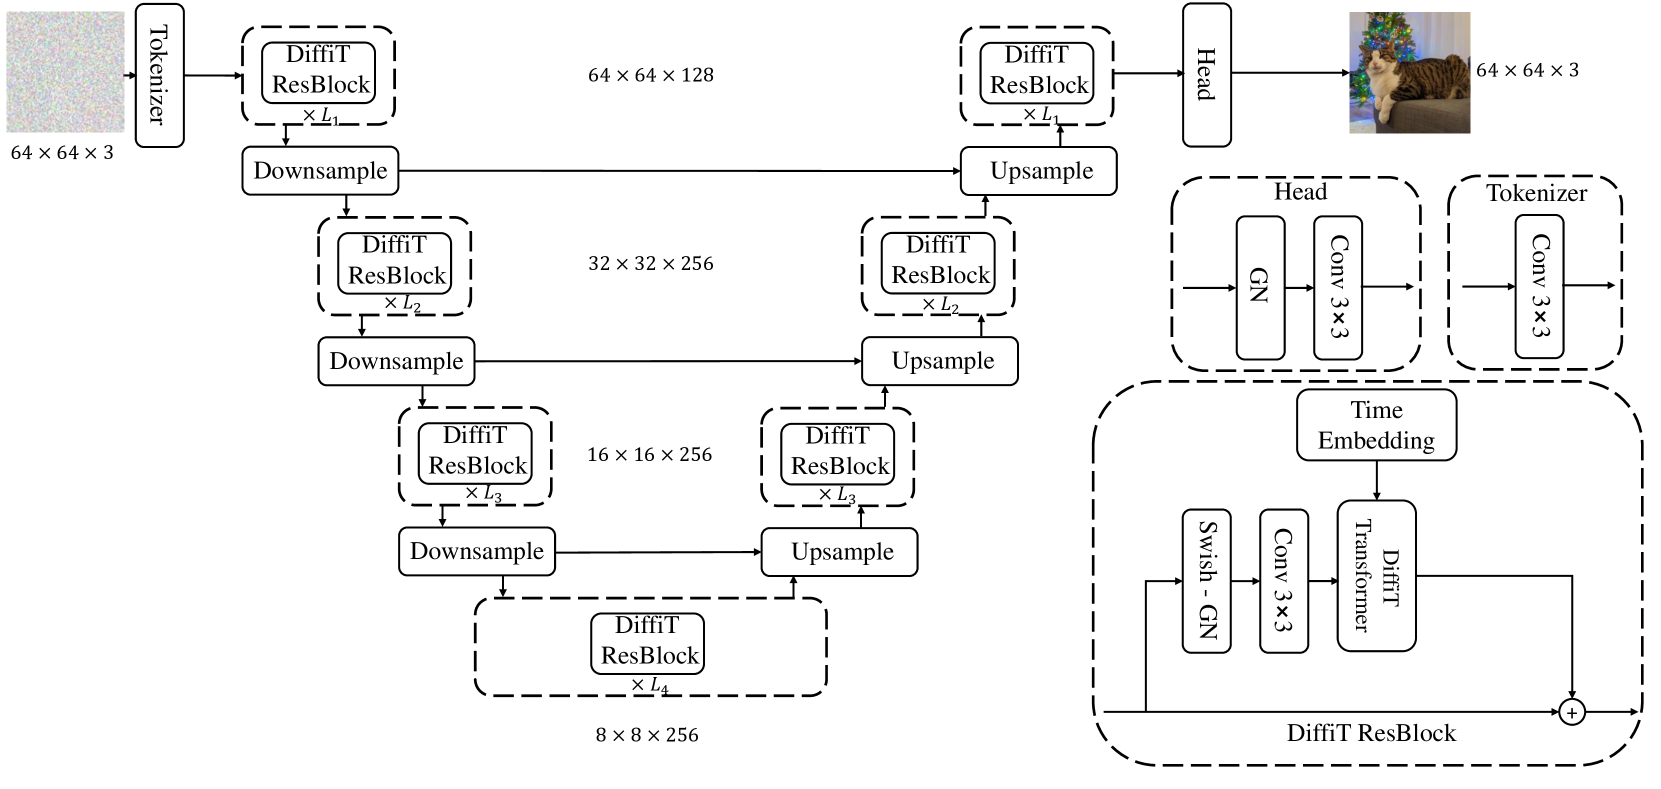
\includegraphics[width=0.9\textwidth]{images/diffit.png}
	\caption[معماری \lr{DiffiT}]{معماری \lr{DiffiT} با بلوک‌های توجه وابسته به زمان (\lr{TMSA}).}
	\label{fig:diffit}
\end{figure}

مدل \lr{LaVin-DiT}\LTRfootnote{Large Vision Diffusion Transformer} ادامه مسیر مقیاس‌پذیری در خانواده \lr{DiT} است و رفتار مدل‌های انتشار بصری را در مقیاس‌های بزرگ‌تر بررسی می‌کند \cite{2411.11505}. این مدل از این جهت در پیشینه قرار می‌گیرد که نشان می‌دهد پرسش اصلی فقط جایگزین کردن \lr{U-Net} با مبدل نیست، بلکه فهم رابطه میان اندازه مدل، حجم محاسبات، کیفیت تولید و هزینه آموزش نیز اهمیت دارد. شکل \ref{fig:lavin_dit} معماری پیشنهادی این مدل را نشان می‌دهد.

\begin{figure}[H]
	\centering
	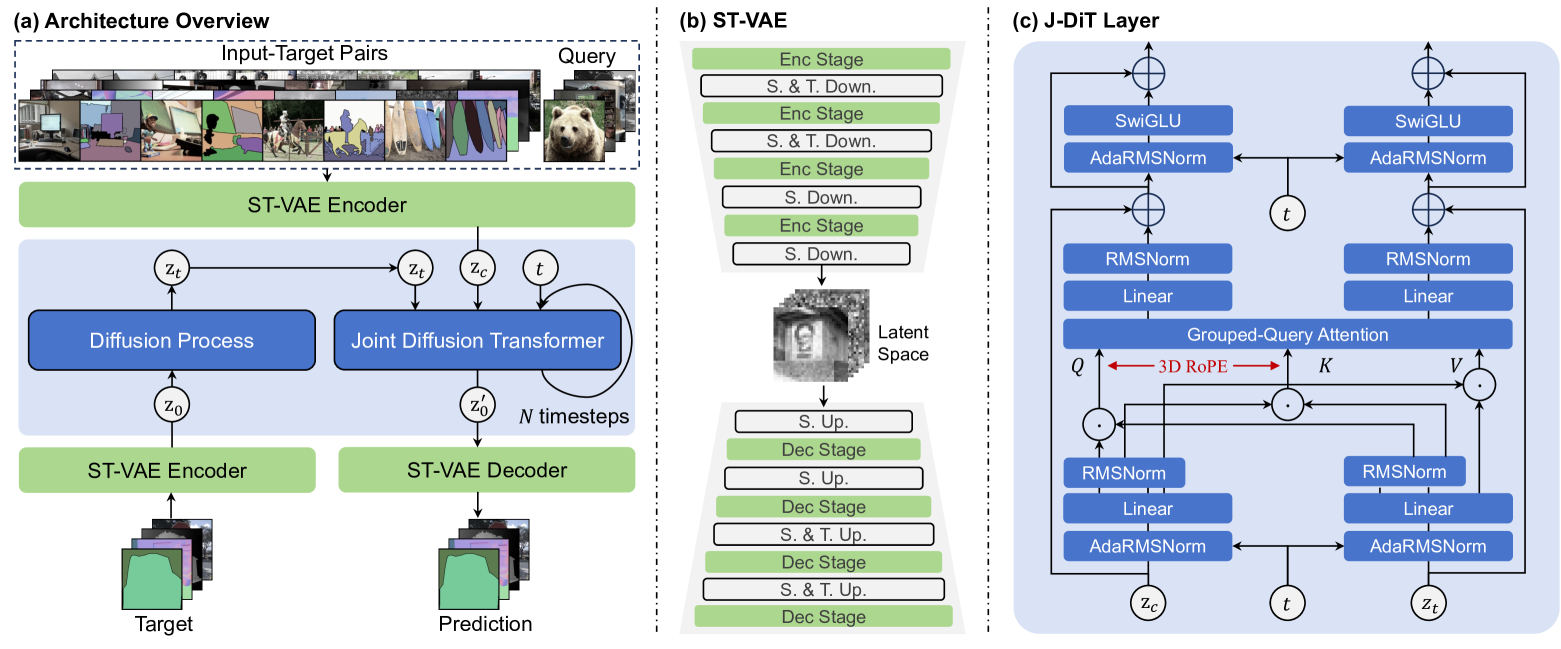
\includegraphics[width=0.9\textwidth]{images/lavin_dit.png}
	\caption[معماری \lr{LaVin-DiT}]{معماری پیشنهادی در \lr{LaVin-DiT} برای بهبود مقیاس‌پذیری \cite{2411.11505}.}
	\label{fig:lavin_dit}
\end{figure}

\lr{LightningDiT} یکی از کارهای جدید در مسیر تقویت مدل‌های انتشار مبتنی بر مبدل است که روی دشواری بهینه‌سازی میان بازسازی نمایش نهان و توان تولید تصویر تمرکز می‌کند \cite{Yao2025LightningDiT}. این کار نشان می‌دهد که در مدل‌های انتشار نهان، کیفیت نهایی فقط به ظرفیت مبدل وابسته نیست، بلکه به تعادل میان کیفیت بازسازی فضای نهان، راهبرد آموزش و مسیر تولید نیز بستگی دارد. از این رو، 
\lr{LightningDiT}
 با بهبود فرایند آموزش مبدل انتشار نهان، به یک مبنای قوی از نظر 
 \lr{FID}
  تبدیل شده است.

\section{روندهای تکمیلی در مدل‌های انتشار مبتنی بر مبدل}

یکی از محورهای اصلی در پیشینه مدل‌های انتشار مبتنی بر مبدل، مسئله مقیاس‌پذیری است. مدل‌های اولیه نشان دادند که با افزایش اندازه شبکه و مقدار محاسبات، کیفیت تولید تصویر بهبود می‌یابد؛ اما این بهبود معمولاً با افزایش شدید هزینه آموزش و استنتاج همراه است. به همین دلیل، پژوهش‌های جدید تلاش کرده‌اند میان ظرفیت مدل، سرعت آموزش و کیفیت نمونه‌های تولیدی تعادل برقرار کنند. برای نمونه، مدل‌های مبتنی بر ماسک‌گذاری و یادگیری با توکن‌های تصویری نشان داده‌اند که می‌توان با کاهش بخشی از محاسبات غیرضروری، آموزش مدل‌های انتشار را سریع‌تر کرد \cite{6822437,2622409}. همچنین چارچوب‌هایی مانند \lr{FiTv2}\LTRfootnote{Flexible Vision Transformer v2}، \lr{EDT}\LTRfootnote{Efficient Diffusion Transformer} و مدل‌های پویای مبدل انتشار، با تغییر طراحی بلوک‌ها، مسیرهای محاسباتی یا سیاست پردازش توکن‌ها تلاش کرده‌اند کیفیت تولید را در کنار کاهش هزینه محاسباتی حفظ کنند \cite{5023251,5439194,7080581,4791247}. در همین امتداد، مدل \lr{Q-DiT}\LTRfootnote{Accurate Post-Training Quantization for Diffusion Transformers} راهکاری برای فشرده‌سازی مدل‌های \lr{DiT} از طریق کوانتیزاسیون پس از آموزش ارائه می‌دهد که در شکل \ref{fig:q_dit} نمایش داده شده است \cite{2406.17343}. این روش با کاهش دقت نمایش وزن‌ها و فعال‌سازی‌ها، بدون نیاز به آموزش مجدد سنگین، کارایی استنتاج را افزایش می‌دهد و نشان می‌دهد که مسئله کارایی تنها به طراحی معماری محدود نیست، بلکه به نحوه نمایش و اجرای پارامترها نیز وابسته است.

\begin{figure}[H]
	\centering
	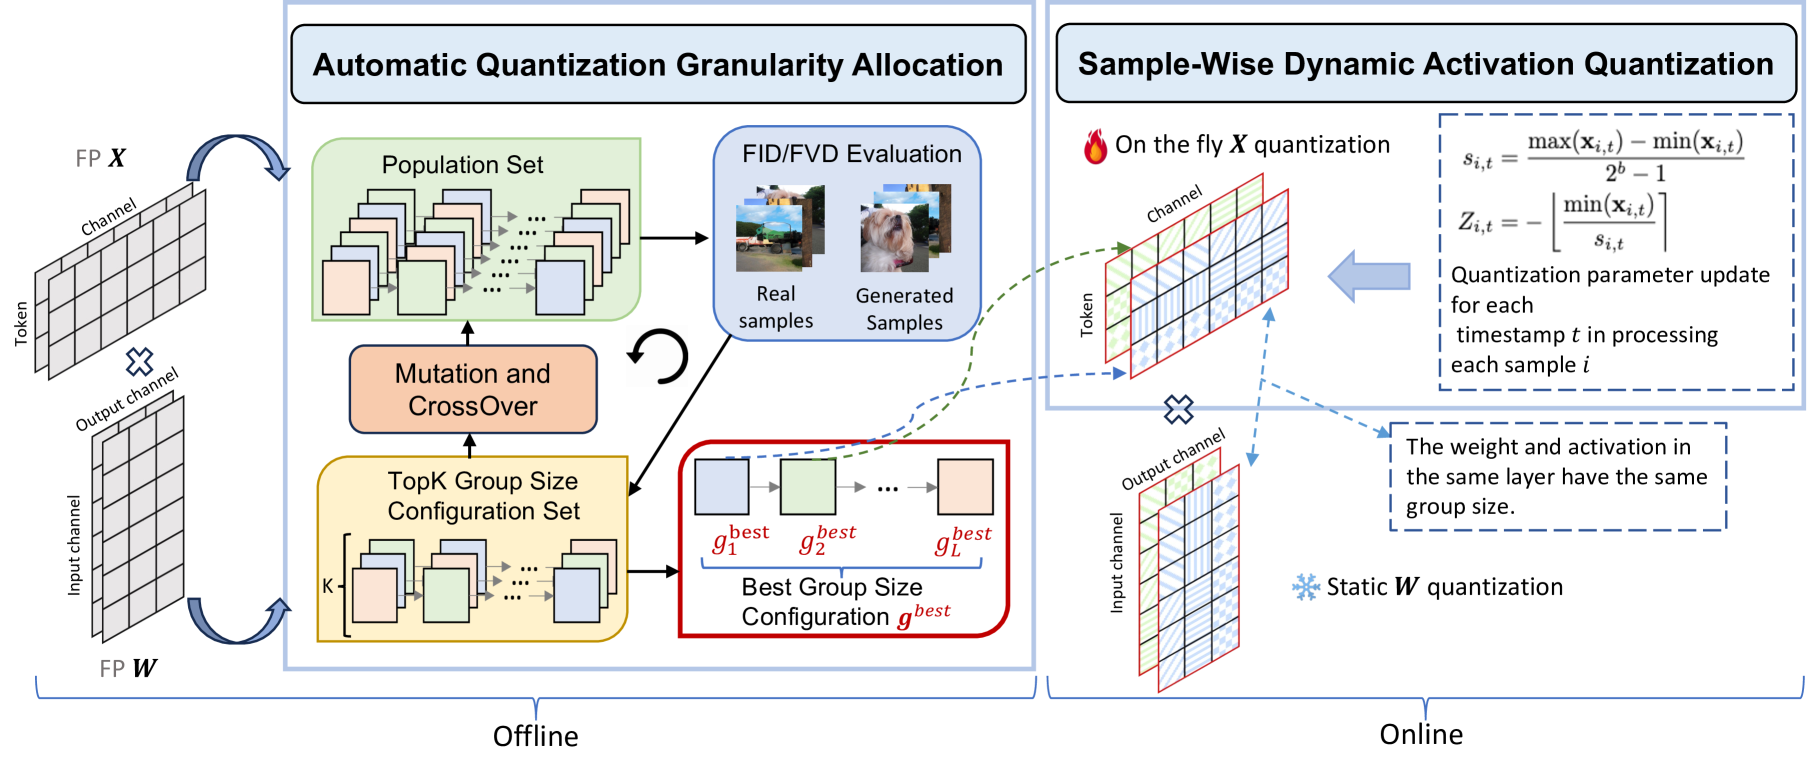
\includegraphics[width=0.9\textwidth]{images/q_dit.png}
	\caption[روش کوانتیزاسیون در \lr{Q-DiT}]{شماتیک روش کوانتیزاسیون در \lr{Q-DiT} \cite{2406.17343}.}
	\label{fig:q_dit}
\end{figure}

در تولید تصویر با وضوح بالا، چالش فقط افزایش تعداد پارامترها نیست؛ بلکه حفظ جزئیات محلی، جلوگیری از اعوجاج و مدیریت وابستگی‌های چندمقیاسی نیز اهمیت دارد. مدل‌هایی مانند \lr{PixArt-Alpha} و نسخه پیشرفته‌تر آن \lr{PixArt-Sigma} با تمرکز بر آموزش کارآمد مبدل‌های انتشار نشان دادند که می‌توان با طراحی مناسب داده، شرط‌گذاری متنی و سازمان‌دهی توکن‌ها، تولید متن-به-تصویر را در وضوح‌های بالا بهبود داد \cite{1031742,chen2024pixartsigma}. همچنین چارچوب‌های مبتنی بر \lr{Rectified Flow}، از جمله مدل مورد استفاده در نسل سوم \lr{Stable Diffusion} و معماری \lr{MM-DiT}\LTRfootnote{Multimodal Diffusion Transformer}، با استفاده از مبدل‌های مقیاس‌پذیر و پردازش جداگانه اطلاعات تصویری و متنی، مسیر دیگری برای تولید تصاویر با کیفیت بالا فراهم کرده‌اند \cite{9168840}. از سوی دیگر، روش‌های چندوضوحی و زمان‌وابسته نشان داده‌اند که کنترل بهتر اطلاعات در سطوح مکانی مختلف می‌تواند به کاهش اعوجاج و بازسازی بهتر ساختارهای تصویری کمک کند \cite{3520873}. این جهت‌گیری‌ها از نظر مفهومی با انگیزه این پژوهش همسو هستند، زیرا معماری پیشنهادی نیز تلاش می‌کند با افزودن شاخه‌ای سبک و وضوح‌بالا، جزئیات مکانی را بدون آموزش مجدد کل مدل تقویت کند.

\subsection{تولید شرطی}
بخش مهم دیگری از پیشینه، به کنترل‌پذیری و شخصی‌سازی مدل‌های انتشار مربوط است. مدل‌های ترکیبی نشان داده‌اند که می‌توان چندین شرط یا مفهوم بصری را در فرایند تولید با یکدیگر ترکیب کرد و از این طریق کنترل معنایی دقیق‌تری بر خروجی به دست آورد \cite{1705308}. روش‌های مبتنی بر مدولاسیون توجه نیز برای تولید متن-به-تصویر متراکم و کنترل‌شده استفاده شده‌اند و نشان داده‌اند که تغییر در نقشه‌های توجه می‌تواند روی جای‌گذاری و انسجام اجزای تصویر اثرگذار باشد \cite{8501335}. همچنین پژوهش‌هایی مانند یادگیری درون‌متنی برای مدل‌های انتشار، تولید شخصی‌سازی‌شده بدون تنظیم زمان آزمون، و تزریق سبک، نشان می‌دهند که سازگار کردن مدل‌های بزرگ با مفهوم یا سبک جدید، یکی از مسائل فعال و مهم در تولید تصویر است \cite{3341281,3521746,3031821}. این روند با بحث هدایت تولید در بخش \ref{sec:ch2-diffusion-frameworks} پیوستگی دارد، زیرا کنترل‌پذیری در عمل به ترکیب شرط‌گذاری، نمونه‌برداری و معماری شبکه حذف نویز وابسته است.

\subsection{کاربردها}
مدل‌های انتشار علاوه بر تصویر دوبعدی، به حوزه‌هایی مانند ویدئو، داده‌های سه‌بعدی و تصویر پزشکی نیز گسترش یافته‌اند. در تولید ویدئو، مدل‌هایی مانند \lr{Video Diffusion Models}، \lr{LaVie} و \lr{Latte} نشان داده‌اند که چالش اصلی، حفظ سازگاری زمانی در کنار کیفیت بصری فریم‌ها است \cite{8313484,8303733,4875773}. در حوزه سه‌بعدی نیز پژوهش‌هایی مانند ویرایش سه‌بعدی فعال‌سازی‌های مدل‌های انتشار یا تولید تصویر استریو نشان می‌دهند که بازنمایی‌های آموخته‌شده در مدل‌های انتشار می‌توانند به فراتر از تولید تصویر دوبعدی تعمیم یابند \cite{9485734,6927085}. همچنین در کاربردهای پزشکی و علمی، تولید تصاویر اخترفیزیکی، سنتز \lr{CT}\LTRfootnote{Computed Tomography} و تحلیل تصاویر بافت‌شناسی نمونه‌هایی از استفاده مدل‌های مولد و مبدل‌ها در دامنه‌های تخصصی هستند \cite{9010310,7223480,4920207}. این گسترش کاربردها نشان می‌دهد که روش‌های سبک و قابل تنظیم، برای انتقال مدل‌های بزرگ به دامنه‌های جدید اهمیت زیادی دارند.

در همین امتداد، مدل \lr{DiT-3D}\LTRfootnote{Three-Dimensional Diffusion Transformer} معماری مبدل‌های انتشار را به تولید \lr{Voxelized Point Clouds} تعمیم می‌دهد \cite{2307.01831}. در این مدل، داده حجمی به پچ‌های سه‌بعدی تقسیم می‌شود و پس از ترکیب با تعبیه‌های موقعیتی سه‌بعدی، به دنباله‌ای از توکن‌ها تبدیل می‌گردد. برای کنترل هزینه محاسباتی ناشی از طول زیاد توکن‌ها در فضای حجمی، \lr{DiT-3D} از توجه پنجره‌ای سه‌بعدی\LTRfootnote{3D Window Attention} استفاده می‌کند و تعاملات را به نواحی محلی محدود می‌سازد. جایگاه این مدل در فصل حاضر بیشتر از زاویه گسترش دامنه کاربرد است، زیرا نشان می‌دهد ایده پچ‌سازی و توجه در \lr{DiT} می‌تواند از تولید تصویر دوبعدی به داده‌های حجمی نیز منتقل شود. این معماری در شکل \ref{fig:dit3d_arch} آمده است.

\begin{figure}[H]
	\centering
	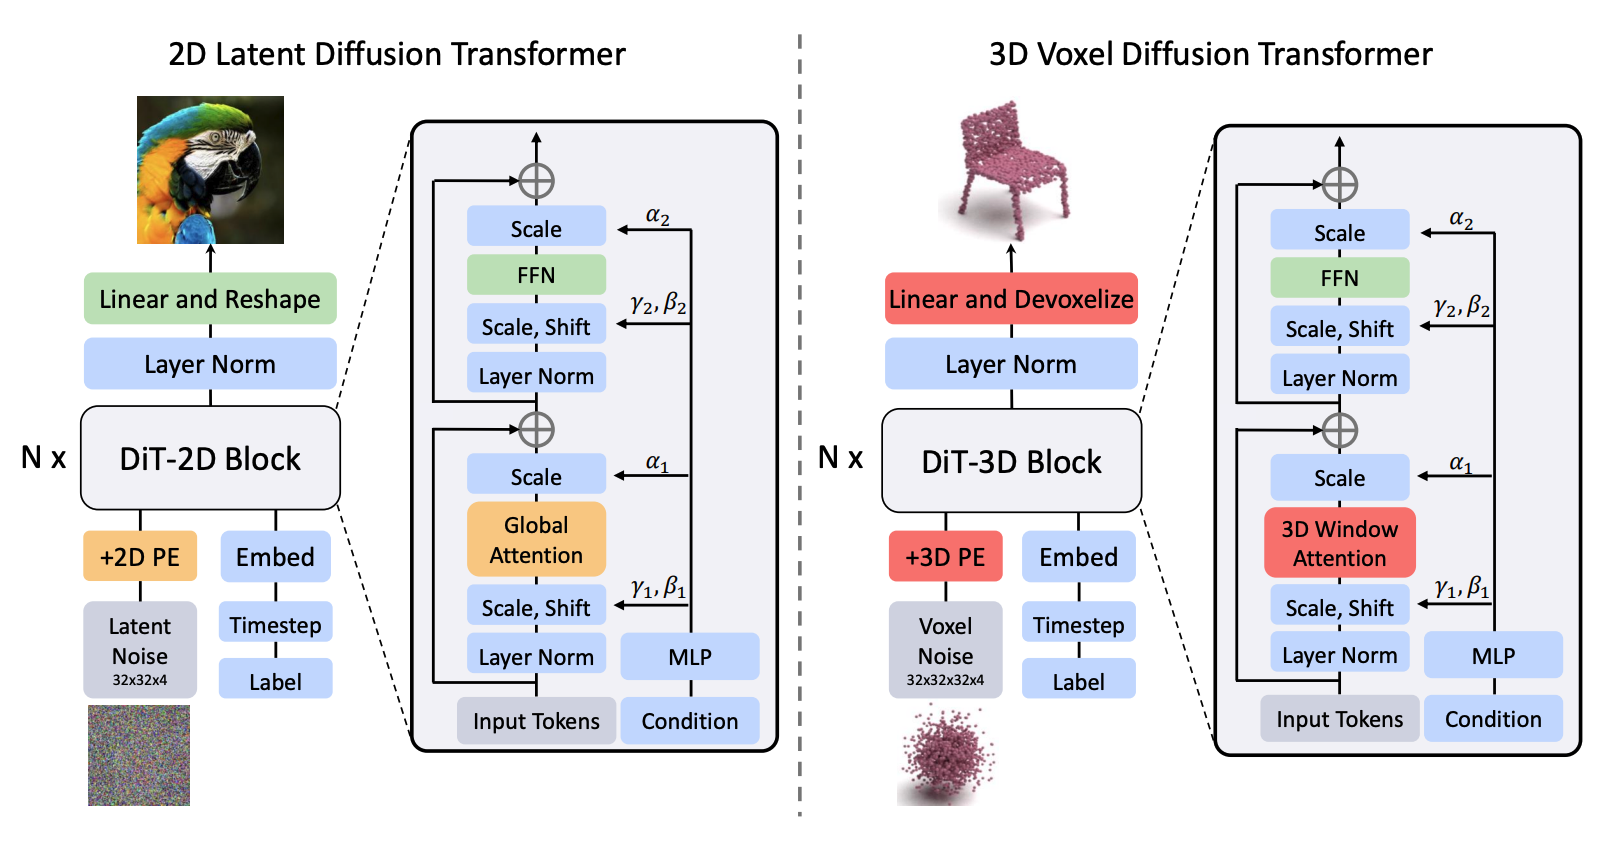
\includegraphics[width=1.0\textwidth]{images/dit_3d.png}
	\caption[معماری \lr{DiT-3D}]{معماری \lr{DiT-3D}: تعمیم مکانیزم پچ‌سازی و توجه به فضای حجمی برای تولید سه‌بعدی \cite{2307.01831}.}
	\label{fig:dit3d_arch}
\end{figure}

\subsection{محلیت و ویژگی‌های ریزدانه}
با وجود قدرت مبدل‌ها در مدل‌سازی وابستگی‌های سراسری، حفظ محلیت و جزئیات ریزدانه همچنان یک مسئله مهم است. پژوهش‌های مربوط به محلیت در مبدل‌های بینایی نشان می‌دهند که نبود سوگیری مکانی محلی می‌تواند در برخی وظایف به ضعف در نمایش بافت‌ها و ساختارهای کوچک منجر شود \cite{0017415}. از سوی دیگر، روش‌هایی که به سازگاری فرکانسی یا تنظیم حافظه‌کارا در مبدل‌های بینایی می‌پردازند، نشان می‌دهند که بخش‌های مختلف طیف فرکانسی و لایه‌های مختلف شبکه نقش یکسانی در انتقال دانش ندارند \cite{7387391,7732706,3649101}.

\section{معماری‌های جریان دوگانه}

استفاده از معماری‌های جریان دوگانه\LTRfootnote{Dual-Stream Architectures} یکی از راهکارهای رایج برای ترکیب اطلاعات سراسری و محلی در پردازش تصویر است. ایده اصلی این رویکرد آن است که یک مسیر شبکه می‌تواند ساختارهای کلی، وابستگی‌های بلندبرد و ویژگی‌های معنایی را مدل کند، در حالی که مسیر دیگر روی جزئیات محلی، لبه‌ها، بافت‌ها و مؤلفه‌های فرکانس بالا تمرکز دارد. برای نمونه، \lr{HRNet}\LTRfootnote{High-Resolution Network} با حفظ نمایش‌های وضوح‌بالا در طول کل فرایند پردازش و تبادل مداوم اطلاعات با شاخه‌های وضوح پایین‌تر، نشان داد که نگه داشتن اطلاعات مکانی دقیق برای وظایفی مانند تشخیص نقاط کلیدی، قطعه‌بندی و بازشناسی بصری اهمیت زیادی دارد \cite{wang2020hrnet}.

شکل \ref{fig:ch2-hrnet-fusion} ایده اصلی \lr{HRNet} را نشان می‌دهد: به‌جای آن‌که شبکه ابتدا نمایش تصویر را به وضوح پایین فشرده و سپس در انتها آن را بازیابی کند، شاخه وضوح‌بالا در تمام مراحل حفظ می‌شود و با شاخه‌های کم‌وضوح‌تر تبادل اطلاعات دارد. این طراحی از نظر مفهومی برای پژوهش حاضر مهم است، زیرا نشان می‌دهد حفظ یک مسیر پرجزئیات می‌تواند مکمل مسیرهای معنایی و کم‌وضوح باشد \cite{wang2020hrnet}.

\begin{figure}[H]
    \centering
    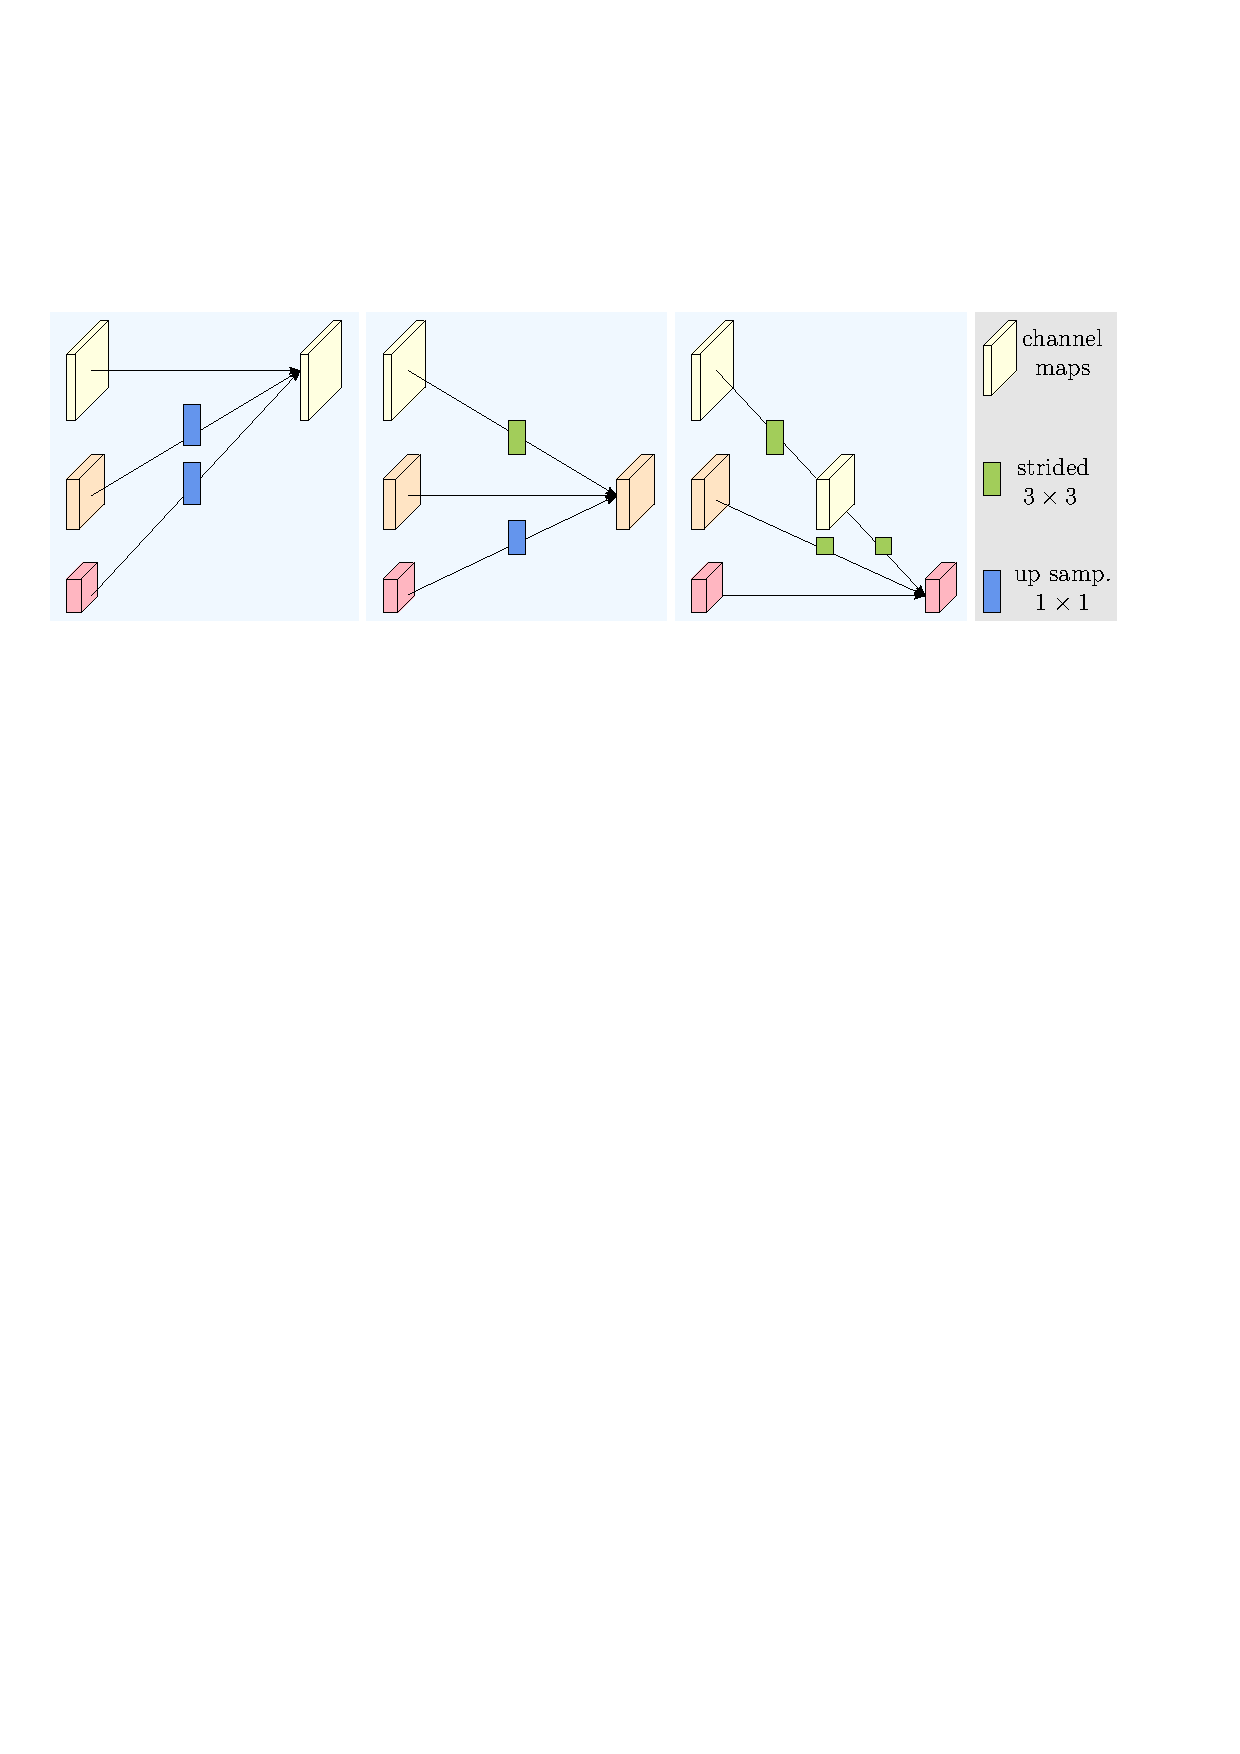
\includegraphics[width=0.92\linewidth]{images/hrnet_multiresolution_fusion.pdf}
    \caption[تجمیع چندوضوحی در \lr{HRNet}]{واحد تجمیع چندوضوحی در \lr{HRNet}: شاخه وضوح‌بالا در کنار شاخه‌های کم‌وضوح‌تر حفظ شده و اطلاعات میان وضوح‌ها به‌صورت مکرر مبادله می‌شود \cite{wang2020hrnet}.}
    \label{fig:ch2-hrnet-fusion}
\end{figure}

در حوزه مبدل‌های بینایی، مدل‌هایی مانند \lr{CrossViT}\LTRfootnote{Cross-Attention Multi-Scale Vision Transformer} این ایده را با استفاده از دو شاخه مبتنی بر اندازه پچ‌های متفاوت پیاده‌سازی کرده‌اند \cite{chen2021crossvit}. در این معماری، که در شکل \ref{fig:ch2-crossvit-architecture} نشان داده شده است، شاخه‌ای با پچ‌های بزرگ‌تر برای دریافت زمینه سراسری و شاخه‌ای با پچ‌های کوچک‌تر برای استخراج جزئیات محلی به کار می‌رود. سپس اطلاعات دو شاخه با سازوکار توجه متقابل میان توکن‌های خلاصه‌ساز مبادله می‌شود. پژوهش‌های مرتبط با طراحی مبدل‌های چندمقیاسی نیز نشان می‌دهند که افزایش دامنه دریافت\LTRfootnote{Receptive Field} در کنار حفظ مسیرهای محلی، برای تحلیل تصویر با وضوح بالا اهمیت کلیدی دارد \cite{3153255,0017415}. همچنین در مدل‌های انتشار مبتنی بر مبدل مانند \lr{U-ViT}، استفاده از مسیرهای چندسطحی و اتصالات بلندبرد، کارایی مشابهی در حفظ اطلاعات جزئیات ایجاد می‌کند \cite{2209.12152}.

\begin{figure}[H]
    \centering
    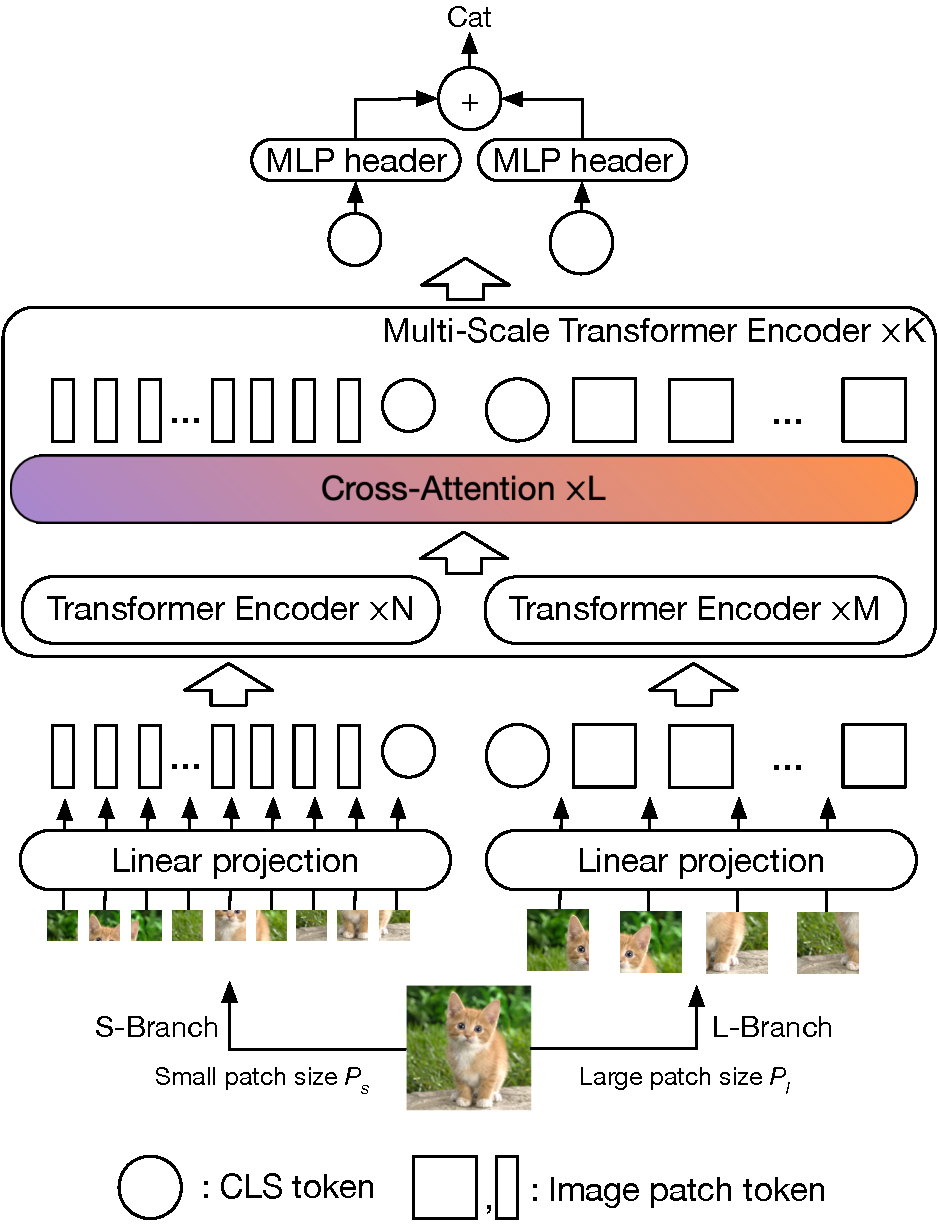
\includegraphics[width=0.96\linewidth]{images/crossvit_architecture.pdf}
    \caption[معماری دوجریانی \lr{CrossViT}]{معماری دوجریانی \lr{CrossViT}: شاخه پچ‌های بزرگ‌تر زمینه سراسری را مدل می‌کند و شاخه پچ‌های کوچک‌تر جزئیات محلی را حفظ می‌کند؛ تبادل اطلاعات میان دو شاخه از طریق توجه متقابل انجام می‌شود \cite{chen2021crossvit}.}
    \label{fig:ch2-crossvit-architecture}
\end{figure}

در \lr{CrossViT} چند راهبرد برای ادغام دو شاخه بررسی شده است: ادغام کامل همه توکن‌ها، ادغام توکن‌های کلاس، ادغام مکانی جفت‌به‌جفت، و ادغام مبتنی بر توجه متقابل. نتیجه مهم این مقایسه آن است که برای انتقال اطلاعات چندمقیاسی الزاماً نیازی به ترکیب پرهزینه همه توکن‌ها نیست؛ گاهی یک توکن خلاصه‌ساز می‌تواند نقش واسط فشرده و کارآمدی میان شاخه‌ها داشته باشد. شکل \ref{fig:ch2-crossvit-fusion} این تفاوت را به‌صورت شماتیک نشان می‌دهد \cite{chen2021crossvit}.

\begin{figure}[H]
    \centering
    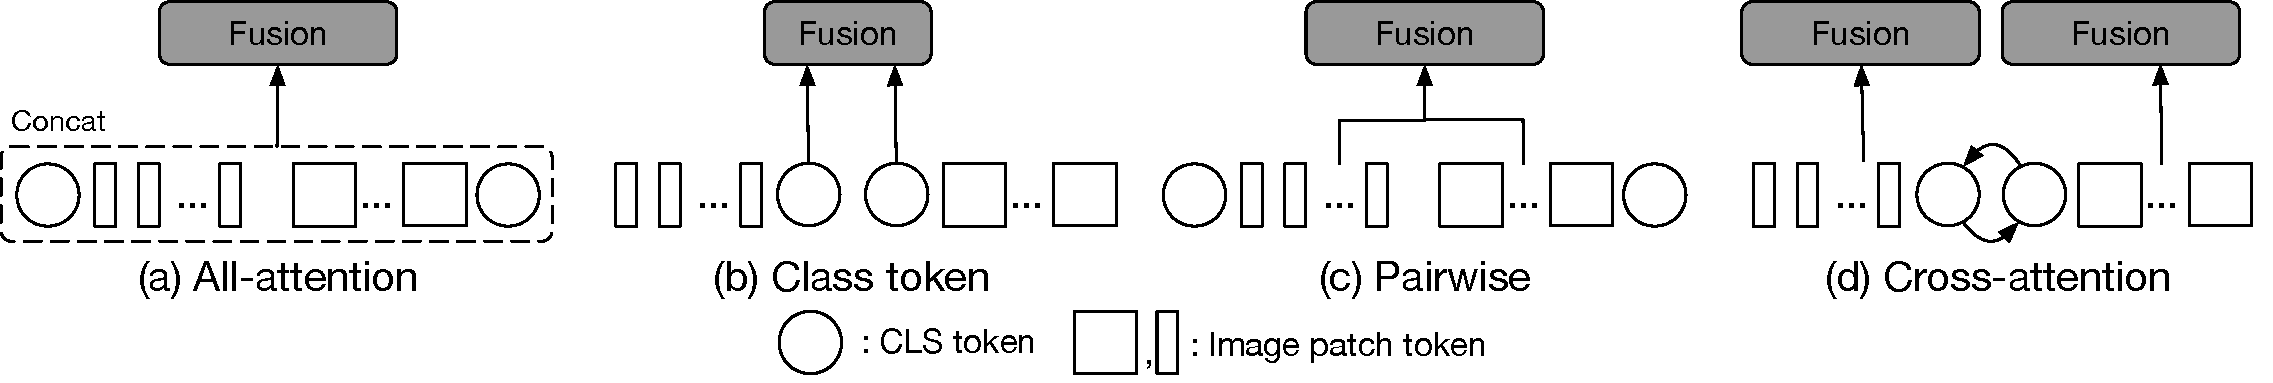
\includegraphics[width=0.9\linewidth]{images/crossvit_fusion_strategies.pdf}
    \caption[\hspace{6pt}راهبردهای ادغام ویژگی در \lr{CrossViT}]{راهبردهای مختلف ادغام ویژگی در \lr{CrossViT}، از ادغام همه توکن‌ها تا توجه متقابل مبتنی بر توکن کلاس \cite{chen2021crossvit}.}
    \label{fig:ch2-crossvit-fusion}
\end{figure}

در سمت مدل‌های انتشار، بازگشت کوتاه به \lr{U-ViT} از زاویه معرفی مدل نیست، بلکه از زاویه حفظ اطلاعات چندسطحی است. همان‌طور که در شکل \ref{fig:uvit} دیده می‌شود، اتصالات بلند میان بلوک‌های ابتدایی و انتهایی مبدل کمک می‌کنند اطلاعات سطح پایین و جزئیات مکانی در مسیر حذف نویز از بین نروند. این نکته، پیوند مستقیمی میان ایده‌های جریان دوگانه و نیاز مدل‌های انتشار به حفظ جزئیات محلی ایجاد می‌کند \cite{2209.12152}.


جدول \ref{tab:ch2-dual-stream-refs} خلاصه می‌کند که هر یک از این معماری‌ها چه نوع مسیری برای حفظ اطلاعات محلی یا چندمقیاسی ایجاد می‌کنند. در هر سه نمونه، یک مسیر کم‌هزینه برای نگه‌داری یا انتقال اطلاعات ریزدانه در کنار مسیر اصلی دیده می‌شود؛ تفاوت در آن است که \lr{HRNet} این کار را با شاخه‌های وضوح متفاوت، \lr{CrossViT} با شاخه‌های پچی متفاوت و توجه متقابل، و \lr{U-ViT} با اتصالات بلند میان لایه‌های مبدل انجام می‌دهد \cite{wang2020hrnet,chen2021crossvit,2209.12152}.

\begin{table}[htbp]
    \centering
    \caption[مقایسه معماری‌های جریان دوگانه]{مقایسه معماری‌های جریان دوگانه}
    \label{tab:ch2-dual-stream-refs}
    \resizebox{\textwidth}{!}{%
    \begin{tabular}{p{0.22\textwidth}p{0.38\textwidth}p{0.32\textwidth}}
        \hline
        \textbf{معماری} & \textbf{مکانیزم اصلی} & \textbf{نوع اطلاعات حفظ‌شده} \\
        \hline
        \lr{HRNet} & نگه‌داری هم‌زمان شاخه‌های وضوح بالا و پایین با تجمیع چندوضوحی تکرارشونده & جزئیات مکانی، لبه‌ها و بافت‌های محلی \\
        \lr{CrossViT} & دو شاخه با اندازه پچ متفاوت و تبادل اطلاعات از طریق توکن‌های کلاس و توجه متقابل & زمینه سراسری در کنار جزئیات ریزدانه مبتنی بر پچ‌های کوچک‌تر \\
        \lr{U-ViT} & اتصال‌های بلند میان بلوک‌های ابتدایی و انتهایی مبدل در شبکه انتشار & اطلاعات سطح پایین و چندمرحله‌ای در مسیر حذف نویز \\
        \hline
    \end{tabular}%
    }
\end{table}

این شواهد نشان می‌دهند که ترکیب هم‌زمان ویژگی‌های درشت‌دانه و ریزدانه می‌تواند برای پردازش تصاویر با وضوح بالا مفید باشد.

\section{تجمیع ویژگی و توکن}
در معماری استاندارد مبدل بینایی، یک توکن ویژه به نام توکن کلاس\LTRfootnote{Class Token} به ابتدای توالی ورودی افزوده می‌شود تا در طول لایه‌های توجه، اطلاعات کل تصویر را به‌صورت فشرده در خود تجمیع کند \cite{Dosovitskiy2020}. این توکن برای وظایفی مانند طبقه‌بندی تصویر مناسب است، زیرا مدل در پایان می‌تواند بازنمایی سراسری تصویر را از آن استخراج کند. با این حال، در معماری‌های چندشاخه یا جریان دوگانه، یک توکن سراسری واحد همیشه برای حفظ جزئیات محلی کافی نیست؛ زیرا ممکن است هنگام فشرده‌سازی کل تصویر، بخشی از اطلاعات ریزدانه و مکانی از دست برود.

راهبرد توکن‌های کلاس محلی بر این ایده استوار است که به‌جای استفاده از یک توکن خلاصه‌ساز برای کل تصویر، می‌توان برای هر ناحیه یا گروهی از توکن‌ها یک توکن خلاصه‌ساز جداگانه تعریف کرد. اگر نمایش محلی توکن‌ها را با $X_l$ نشان دهیم، توکن محلی می‌تواند در نقش «پرس‌وجو» ($Q$) عمل کند و اطلاعات مهم را از «کلیدها» ($K$) و «مقادیر» ($V$) متناظر با همان گروه استخراج کند. محاسبه توجه در این حالت همان رابطه \ref{eq:scaled-dot-product-attention} است، اما $Q$، $K$ و $V$ فقط از توکن‌های همان گروه محلی ساخته می‌شوند \cite{Dosovitskiy2020,chen2021crossvit}.
سازوکارهای مشابه در معماری‌هایی مانند \lr{CrossViT} برای تبادل اطلاعات میان شاخه‌های چندمقیاسی استفاده شده‌اند؛ نمونه‌ای از این سازوکار در شکل \ref{fig:ch2-crossvit-ca-module} آمده است \cite{chen2021crossvit}.

\begin{figure}[H]
    \centering
    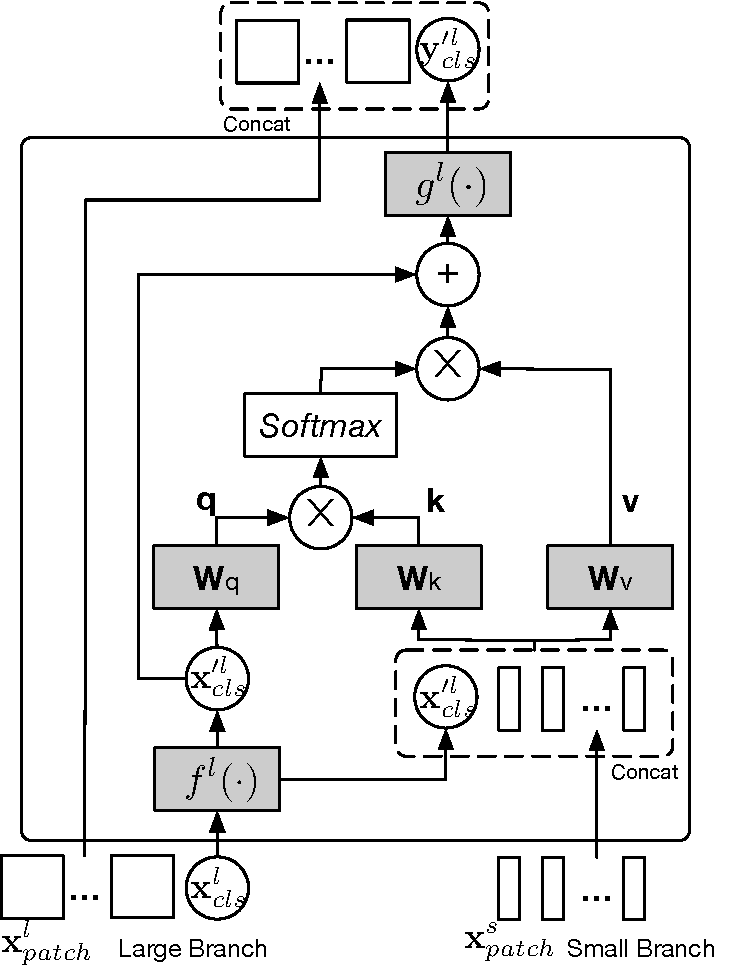
\includegraphics[width=0.9\linewidth]{images/crossvit_cross_attention_module.pdf}
    \caption[\hspace{6pt}ماژول توجه متقابل در \lr{CrossViT}]{ماژول توجه متقابل در \lr{CrossViT}: توکن کلاس یک شاخه نقش پرس‌وجو را دارد و اطلاعات را از توکن‌های شاخه دیگر دریافت می‌کند \cite{chen2021crossvit}.}
    \label{fig:ch2-crossvit-ca-module}
\end{figure}

\section{روش‌های تنظیم دقیق}

\label{sec:full_finetuning} تنظیم دقیق کامل به عنوان رویکرد پایه در تغییر رفتار مدل‌های بزرگ، شامل آزادسازی و به‌روزرسانی تمام پارامترهای شبکه در طول آموزش روی وظیفه یا دامنه هدف است. این فرآیند نسبت به روش‌های تنظیم دقیق پارامتر-کارا، پیچیدگی و هزینه بسیار بیشتری دارد چرا که شبکه‌های امروزی ممکن است دارای میلیاردها پارامتر باشند. همین ویژگی موجب مصرف بالای حافظه \lr{GPU}\LTRfootnote{Graphics Processing Unit}،
 نیاز به ذخیره‌سازی فعال‌سازی‌ها برای کل لایه‌ها، و افزایش زمان هر گام یادگیری می‌شود 
 \cite{5294562}.

\subsection{تنظیم دقیق پارامتر-کارا}
\label{sec:efficient_parameter_finetuning} تنظیم دقیق پارامتر-کارا در سال‌های اخیر به عنوان پاسخی عملی به محدودیت‌های زمان و منابع موردنیاز برای آموزش مدل‌های بزرگ مطرح شده است. ایده اصلی کاهش تعداد پارامترهایی است که طی فرآیند تنظیم دقیق به‌روز می‌شوند تا فشار حافظه، هزینه محاسباتی و مدت زمان آموزش کمتر شود، در حالی که کیفیت خروجی در سطح رقابتی باقی بماند \cite{8409325}. 
در این رویکردها بخش اعظم وزن‌های شبکه ثابت نگه داشته شده و تنها مجموعه کوچکی از پارامترهای افزوده‌شده یا انتخاب‌شده برای یادگیری آزاد هستند. 
\lr{FineDiffusion} یک روش تنظیم دقیق پارامتر-کارا برای تولید تصویر شرطی ریزدانه است که مسئله مقیاس‌پذیری تولید کلاسی را در تعداد زیاد کلاس‌ها بررسی می‌کند \cite{Pan2024FineDiffusion}. ایده اصلی این روش آن است که برای سازگار کردن مدل انتشار با کلاس‌های ریزدانه، لازم نیست همه وزن‌های شبکه آزاد شوند؛ در عوض می‌توان بخش محدودی از پارامترهای مؤثر بر شرط‌گذاری و تطبیق آماری مدل را به‌روزرسانی کرد. این بخش‌ها شامل تعبیه‌های کلاسی، بایاس‌ها و پارامترهای مرتبط با نرمال‌سازی هستند؛ یعنی اجزایی که رفتار شرطی مدل را تغییر می‌دهند، اما بدنه اصلی تولیدکننده را تا حد زیادی حفظ می‌کنند.

% \section{جمع‌بندی}
در این فصل، پیشینه پژوهش‌های مرتبط با معماری پیشنهادی از چهار زاویه بررسی شد. نخست، چارچوب‌های اصلی مدل‌های انتشار و مسیر حرکت آن‌ها به سمت مدل‌های مبتنی بر مبدل توضیح داده شد و نمونه‌هایی مانند \lr{GenViT}، \lr{U-ViT}، \lr{DiT}، \lr{DiffiT}، \lr{LaVin-DiT} و \lr{LightningDiT} نشان دادند که مبدل‌ها می‌توانند به بدنه اصلی مدل‌های انتشار تبدیل شوند. دوم، روندهای تکمیلی حوزه نشان دادند که مقیاس‌پذیری، کارایی، شرط‌پذیری و حفظ جزئیات محلی همچنان چالش‌های مهم این خانواده از مدل‌ها هستند. سوم، معماری‌های جریان دوگانه و چندوضوحی مانند \lr{HRNet} و \lr{CrossViT} نشان دادند که ترکیب یک مسیر سراسری با مسیری محلی می‌تواند راهکاری مؤثر برای حفظ جزئیات ریزدانه باشد. چهارم، روش‌های تنظیم دقیق پارامتر-کارا، به‌ویژه \lr{FineDiffusion}، نشان دادند که می‌توان بدون به‌روزرسانی کامل مدل پایه، مسیرهای جدیدی برای سازگارسازی و تزریق ویژگی ایجاد کرد \cite{0214306,2212.09748,wang2020hrnet,chen2021crossvit,8409325,Pan2024FineDiffusion}.

% بر این اساس، شکاف پژوهشی این پایان‌نامه در نقطه اتصال این چهار محور قرار می‌گیرد: استفاده از یک بدنه اصلی \lr{DiT} برای حفظ دانش سراسری، افزودن یک شاخه وضوح‌بالا برای استخراج ویژگی‌های محلی، به‌کارگیری توکن‌های کلاس محلی برای تجمیع هوشمند ویژگی‌ها، و آموزش تنها بخش کوچکی از پارامترها برای کاهش هزینه تنظیم دقیق. فصل بعد معماری پیشنهادی \lr{DuoDiT} را بر پایه همین منطق معرفی می‌کند.
